\documentclass{../template/Report}%方括号内写yuxi即生成预习报告\documentclass[yuxi]{../template/Report}
\settemplatedir{../template/}%设置模板路径
\usepackage{wrapfig}
\exname{分光计的调整和使用} %实验名称
\extable{18} %实验桌号
\instructor{何至} %指导教师
\class{信工2401} %班级
\name{姚舜瑜} %姓名
\stuid{3240100532} %学号

\nyear{2025} %年
\nmonth{12} %月
\nday{9} %日
\nweekday{二} %星期几，e.g. \nweekday{三}
\daypart{上午}%上午/下午

\redate{} %如有实验补做，补做日期
\resitu{} %情况说明：

\begin{document}
\maketitle%输出封面
\section{预习测试（10分）}
上课前到学在浙大上完成，注意测试仅1次机会。期末时测试分数会与报告其它部分的分数进行加和处理。
\section{原始数据（20分）}
\begin{figure}[H]
  \centering
  
\includegraphics[width=0.8\textwidth]{figures/原始数据.jpg}
  \caption{原始实验数据}
\end{figure}
\section{结果与分析}
\subsection{数据处理与结果（30分）}
\begin{table}[H]
\centering
\caption{数据处理与结果}
\label{tab:data}
\resizebox{.95\textwidth}{!}{
\begin{tabular}{|l|cc|cc|c|c|c|}
\hline
\multirow{2}{*}{\begin{tabular}[c]{@{}l@{}}实验\\ 次数\end{tabular}} &
  \multicolumn{2}{c|}{方位左} &
  \multicolumn{2}{c|}{方位右} &
  \multirow{2}{*}{$\left|\theta_\text{左I} - \theta_\text{右I}\right|$} &
  \multicolumn{1}{l|}{\multirow{2}{*}{$\left|\theta_\text{左II} - \theta_\text{右II}\right|$}} &
  \multicolumn{1}{l|}{\multirow{2}{*}{$\angle A$}} \\ \cline{2-5}
 &
  \multicolumn{1}{c|}{\begin{tabular}[c]{@{}c@{}}游标I窗\\ $\theta_\text{左I}$\end{tabular}} &
  \begin{tabular}[c]{@{}c@{}}游标II窗\\ $\theta_\text{左II}$\end{tabular} &
  \multicolumn{1}{c|}{\begin{tabular}[c]{@{}c@{}}游标I窗\\ $\theta_\text{右I}$\end{tabular}} &
  \begin{tabular}[c]{@{}c@{}}游标II窗\\ $\theta_\text{右II}$\end{tabular} &
   &
  \multicolumn{1}{l|}{} &
  \multicolumn{1}{l|}{} \\ \hline
1 & \multicolumn{1}{c|}{\ang{354;55}} & \ang{174;55} & \multicolumn{1}{c|}{\ang{235;10}} & \ang{55;2} & \ang{119;45} & \ang{119;53} & \ang{59;54} \\ \hline
2 & \multicolumn{1}{c|}{\ang{356;15}}   & \ang{176;20} & \multicolumn{1}{c|}{\ang{236;24}} & \ang{56;20}  & \ang{119;51} & \ang{120;0} & \ang{59;58} \\ \hline
3 & \multicolumn{1}{c|}{\ang{358;40}}  & \ang{178;40}  & \multicolumn{1}{c|}{\ang{238;49}} & \ang{58;50}   & \ang{119;51} & \ang{119;50} & \ang{59;55} \\ \hline
4 & \multicolumn{1}{c|}{\ang{360;55}} & \ang{180;50} & \multicolumn{1}{c|}{\ang{239;50}} & \ang{59;20}  & \ang{121;5} & \ang{121;30} & \ang{60;39} \\ \hline
5 & \multicolumn{1}{c|}{\ang{354;30}} & \ang{174;31} & \multicolumn{1}{c|}{\ang{234;30}} & \ang{54;30}  & \ang{120;0} & \ang{120;1} & \ang{60;0} \\ \hline
6 & \multicolumn{1}{c|}{\ang{355;49}}  & \ang{175;50} & \multicolumn{1}{c|}{\ang{236;0}}  & \ang{56;1}   & \ang{119;49} & \ang{119;49} & \ang{59;54} \\ \hline
\end{tabular}
}
\end{table}
$\angle A$平均值：$\bar{\angle A}$ = $\dfrac{\displaystyle\sum_{i=1}^6 \angle A_i}{6} =\dfrac{\ang{59;54}+\ang{59;58}+\ang{59;55}+\ang{60;39}+\ang{60;0}+\ang{59;54}}{6} = \ang{60;3}$
\subsection{误差分析（20分）}
\subsubsection{不确定度计算}
\paragraph{A类不确定度：}
如果有$n$组数据，则A类不确定度的计算方法为:
\[
u_A = \sqrt{\dfrac{1}{n \cdot (n - 1)} \cdot \sum_{i = 1}^n (x_i - \bar{x})^2}
\]
带入数据
\[
u_A = \sqrt{\frac{1}{6 \cdot (6 - 1)} \cdot \left[(\ang{59;54} - \ang{60;3})^2 + \cdots + (\ang{60;39} - \ang{60;3})^2\right]} = \ang{;7.2;}
\]
\paragraph{B类不确定度：}
因为游标读数估计误差为$\pm\ang{0;1}$，故B类不确定度为
\[
u_B = \frac{\Delta_\text{仪}}{\sqrt{3}} = \frac{1}{\sqrt{3}}\ang{;1} = \ang{;0.6;}
\]
\paragraph{合成不确定度：}
\[
u = \sqrt{u_A^2 + u_B^2} = \sqrt{\ang{;7.2;}^2 + \ang{;0.6;}^2} \approx \ang{;7;}
\]
\paragraph{最终结果表达式}
\[\boxed{\angle A = \ang{60;3} \pm \ang{;7;}}\]
\setlist[enumerate]{leftmargin=2em}
\subsubsection{误差原因分析：}
\begin{enumerate}[label=(\arabic*)]
    \item \textbf{对准误差：} 这是最主要的误差来源。人眼判断望远镜分划板竖线是否严格对准反射像中心存在主观性，且反射像本身具有一定宽度，导致读数存在分散性。
    \item \textbf{调节误差：} 实验前的“各半调节法”可能未达到完美状态，即望远镜光轴与仪器主轴、载物台平面与仪器主轴并未严格垂直，导致反射光线不在同一水平面上，引入测量误差。
    \item \textbf{环境与操作因素：} 锁紧螺钉若未完全锁死，在转动望远镜或读数时可能引起仪器微小位移；外界光线干扰也可能影响对反射像清晰度的判断。
\end{enumerate}
\subsection{实验探讨（10分）}
本实验成功地利用了分光计测量了三棱镜的顶角。在理论层面，我加深了对光的折射和反射原理的理解，了解了分光计的工作原理及其在光学测量中的应用。在实验操作层面，我掌握了分光计的调节方法，如各半调节法，学会了如何准确读数以减少误差。此外，通过数据处理，我体会到了不确定度分析的重要性。
\section{思考题（10分）}
\subsection{测量三棱镜顶角时，棱镜摆放的位置怎么选，对测量有怎样的影响？}



\begin{wrapfigure}[8]{r}{0.4\textwidth}
  \centering
  \vspace{-10pt}
  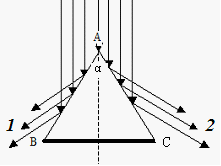
\includegraphics{figures/棱镜位置.png}
  \caption{\small 棱镜位置对光路的影响示意图}
\end{wrapfigure}
{
  \textbf{答：}
测量时，棱镜应当放置在载物台中心略微偏下的位置，并使待测顶角正对平行光管。
\begin{enumerate}
    \item \textbf{位置选择原因：} 选择这个位置是为了保证平行光管射出的光束能够照射到三棱镜两个反射面的中部，而非边缘。
    \item \textbf{对测量的影响：} 如果棱镜位置过于靠上（靠近平行光管），光束可能无法完整照射到反射面，导致反射光线无法进入望远镜；若偏离中心过远，则可能导致其中一个反射面无法接收到光线，从而无法完成测量。
\end{enumerate}
}

\subsection{望远镜观察时有没有发现视差的问题？如有，应怎样解决？若存在视差对测量会有怎样的影响？}
\textbf{答：}
观察时若发现眼睛左右移动时，分划板十字线与观察到的像之间有相对位移，说明存在视差，即像未准确落在分划板平面上。
\begin{enumerate}
    \item \textbf{消除方法：} 先调节目镜使十字线清晰，再调节物镜或移动分划板，使目标像也清晰成像在分划板平面上，直至无相对移动。
    \item \textbf{对测量的影响：} 视差的存在会直接引入读数误差，因为观察角度的微小变化会导致对准位置偏移，影响测量结果的稳定性。
\end{enumerate}

\subsection{当调节载物台与望远镜垂直于分光计的转动主轴时，将双面反射镜置于载物台上，能观测到一侧反射回来的绿十字像，但将载物台转过180度后，望远镜视场内看不到绿十字像，请分析原因。应当怎样调节？}
\textbf{答：}
出现这种情况的原因是载物台平面与分光计转动主轴不平行。虽然在一侧调节使反射光进入了望远镜，但当载物台旋转180度后，载物台的倾斜方向发生反转，导致反射光线在竖直方向偏离，移出了望远镜视场。

调节时应采用“各半调节法”：
\begin{enumerate}
    \item 保持望远镜不动，调节载物台调平螺钉，使反射像向中心横线移动一半距离；
    \item 调节望远镜俯仰螺钉，使像移动剩下的一半距离直至重合。
    \item 反复进行上述步骤，直至旋转180度后像位置不变。
\end{enumerate}
\begin{figure}[H]
  \centering
  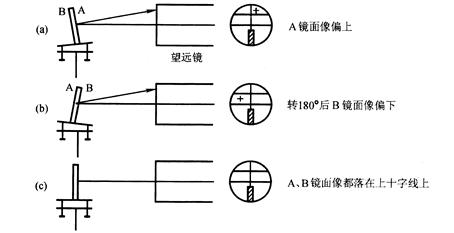
\includegraphics[width=0.7\textwidth]{figures/各半测量.png}
  \caption{光路调节示意图}
\end{figure}
\insertnotes
\end{document}